\documentclass{article}

% Language setting
% Replace `english' with e.g. `spanish' to change the document language
\usepackage[french]{babel}
\usepackage[fleqn]{amsmath} % Aligner les équations à gauche


% Set page size and margins
% Replace `letterpaper' with`a4paper' for UK/EU standard size
\usepackage[letterpaper,top=2cm,bottom=2cm,left=3cm,right=3cm,marginparwidth=1.75cm]{geometry}

% Useful packages
\usepackage{amsmath}
\usepackage{graphicx}
\usepackage{subcaption}
\usepackage[colorlinks=true, allcolors=blue]{hyperref}

\title{TD 13}
\author{IPESUP - PC }
\date{18 Décembre 2024}

\begin{document}
\maketitle

\section{Puits Canadien} Le puits canadien est un système de préchauffage passif de l’air utilisant les réserves d’énergie
du sol entourant la maison. En faisant passer l’air dans une canalisation enterrée dans le
sol, celui-ci se réchauffe, ce qui permet de réduire fortement la consommation électrique de
chauffage en hiver, ainsi que les émissions de $CO_2$, qui en résultent. Dans cet exercice, un
modèle simple de ce dispositif est étudié.
Une entrée d'air est située à une distance $L$ de la maison. Une pompe à l’intérieur de la maison
permet de faire circuler l’air dans un tuyau de section $ S$ enterré à une profondeur $h$ dans le
sol. 



\begin{figure}[h]
  \centering
  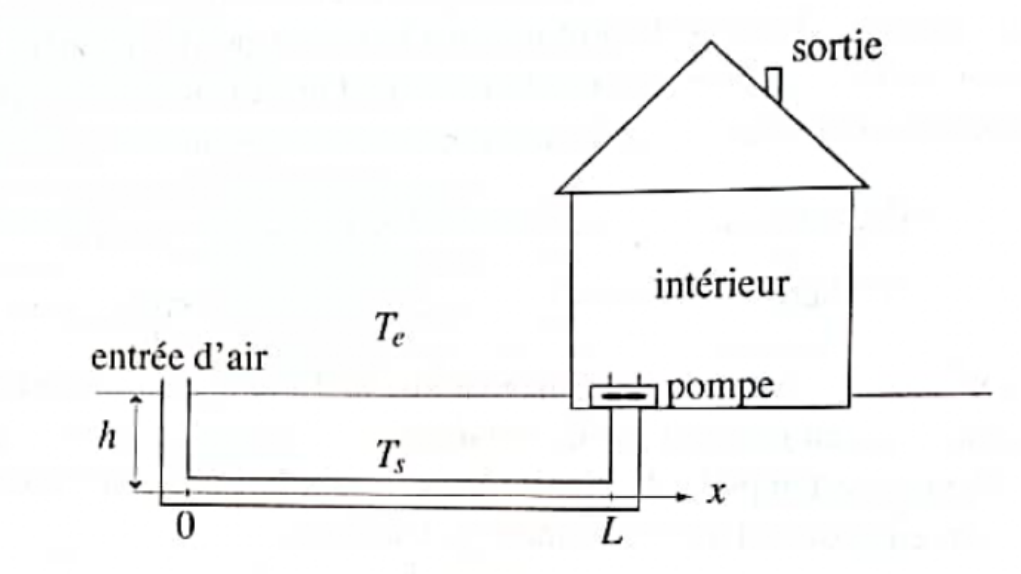
\includegraphics[width=0.4\textwidth]{maison.png}
  \label{fig:maison}
    \caption{Schéma de fonctionnement d'un puits canadien}


\end{figure}


On suppose que les échanges thermiques ne se font que dans la partie horizontale de la canalisation (cylindre de rayon $ R$), comprise entre les abscisses $ x = 0$ et $ x = L$. L’air est considéré comme un gaz parfait de capacité thermique massique à pression constante $c_p$, de masse volumique $\mu$ et de conductivité thermique $\lambda$. On suppose que la température $ T (x)$ est uniforme sur une section droite du tube. L'air se déplace à la vitesse $ v $ constante et uniforme. il entre dans la canalisation  en $ x = O$, à la température $T_e = 10$ °C.

Les échanges thermiques le long de la paroi entre l’air et le sol sont décrits par le flux thermique surfacique : $\Phi = h(T(x)-T_s)$, où $h=$ 6,5 $W.m^{-2}.K^{-1}$
\begin{enumerate}
    \item En supposant que la température extérieure suit la loi $T(0,t) = T_e + T_1 cos(\omega t)$, déterminer la loi de variation de la température dans le sol $T(z,t)$ en la cherchant de la forme $T(z,t) = T_0 + f(z)cos(\omega t - \phi(z))$, avec z la profondeur, nulle à la surface. A quelle profondeur doit-on enterrer la canalisation pour que les variations de température du sol autour de cette dernière soient inférieures à 2°$C$ ? 
    \\
    Dans la suite, on considérera  que la température du sol autour de la canalisation est uniforme et constante et vaut $T_s$
    \item En appliquante le premier principe de la thermodynamique au système fermé constitué de l'air contenu dans la portion de canalisation comprise entre les plans d'abscisse $x$ et $x+dx$ à l'instant $t$, montrer que la température $T(x)$ vérifie l'équation : 
    \begin{equation}
        \frac{d^2T}{dx^2} - \frac{c_p \mu v}{\lambda} \frac{dT}{dx} - \frac{2h}{\lambda R} (T(x)-T_s)=0
    \end{equation}
    \item À quelle condition sur $\lambda$,$L$,$\mu$, $c_p$ et $v$ peut-on  négliger le transfert thermique par diffusion devant le transfert thermique par convection  ? Donner un ordre de grandeur de la vitesse de l'air dans le tuyau pour que cette approximation soit valable. Simplifier alors $(1)$
    \item Résoudre cette équation en faisant apparaitre une longueur caractéristique $\delta$ à exprimer en
fonction des paramètres du problème. 
\item  Établir l’expression littérale de la longueur $L $ de canalisation nécessaire à l’obtention d’une
température d’entrée de l’air dans la maison égale à $T_L$ donnée. Pourquoi le puits permet de
réduire fortement la consommation électrique de chauffage ? Quelle peut être l’utilité du puits
en été (il est appelé également « puits provençal ») ? 
\item  Le volume de la maison est $V = 800 m^3$ , le rayon de la canalisation est $R = 10 cm$, l'air
extérieur est à la température $T_e = 30$°$C$. On veut renouveler l’air de la maison en 2 heures.
Quelle doit être la valeur de la vitesse $ v$ ? 
\item Quelle doit être la longueur de la canalisation pour que la température d’entrée de l’air
dans la maison soit de $20$°$C $ ? \\[1cm]
\end{enumerate}




\section{Fusible}

Un fusible est constitué par un fil conducteur cylindrique homogène, de section droite d’aire
$S$, de longueur utile $ L$, de masse volumique $\mu$ et de capacité thermique massique $c$. Il possède
une conductivité électrique $\gamma$ et une conductivité thermique $K$. Il est traversé par un courant
électrique continu d’intensité $I$. Ce fil est enfermé dans une capsule remplie d’une substance
assurant une isolation thermique et électrique parfaite. Les températures en $x =0 $ et $ x =L$
sont imposées et égales à la température $T_0$ du milieu ambiant.
Pour les applications numériques, on prendra les valeurs suivantes, données dans le système
international d’unités (SD) : $K = 65$ SI ; $\gamma$= 1,2 x 10 SI ; $c$ = 460 SI ; $\mu$ =$ 2,7 \times 10^3 kg.m^{-3}$ ;
$T_0 =290 K$; $L=2,5 cm$. 

\begin{enumerate}
    \item Montrer que la résistance d'un   conducteur cylindrique de conductivité $K$ de longueur
$L$, de section $S$, parcouru par un courant $I$ uniformément réparti et parallèle à son axe, est
$R=\frac{L}{\gamma S}$ On se place en régime permanent. 
\item Établir l’équation différentielle vérifiée par la température $T$. Donner l’expression littérale
de $T(x)$ et représenter graphiquement $T$ en fonction de $x$. 
\item Le matériau constituant le fil fond à $T_f = 390 K$. On veut fabriquer un fusible qui admet
une intensité maximale $I_{max} = 16 A$.
Préciser l’endroit de la rupture en cas de dépassement de $I_{max}$. Déterminer l’expression littérale de l’aire $S$ à prévoir. Faire l’application numérique. 
\item  On fixe $ I = 10 A$. Le fil a la section $S$ trouvée à la question précédente. Evaluer littéralement puis numériquement la puissance thermique $P_{th}(0)$ transférée par conduction en $x= 0$.
Préciser si cette puissance est reçue ou fournie par le fil. Même question pour la puissance
thermique $P_{th}(L)$ transférée en $x = L$. Quelle relation a-t-on entre $P_{th}(0)$, $P_{th}(L)$ et la puissance
électrique $P$ fournie à l’ensemble du fil ? Commenter. 

\end{enumerate}

\section{Durée de survie d'un plongeur }
Un plongeur est équipé de sa combinaison.
On note $T_e$, la température de l’eau environnante, uniforme et constante. La température initiale du plongeur est $T_{i0}$ = 37°C. Les pertes thermiques ont lieu au niveau de la peau et de la
combinaison. 
\begin{enumerate}
    \item Rappeler l’expression de la résistance thermique dans le cas d’un modèle unidimensionnel,
en fonction de la section $S$, de l’épaisseur $e$ et de la conductivité thermique $\gamma$.
\item On modélise les pertes par convection par un flux thermique surfacique $\Phi = Sh(T-T_e)$
Quelle résistance $R_c$ peut-on associer aux pertes par convection ? 
\item  On modèlise les pertes par rayonnement par un flux thermique surfacique $\Phi_r = \sigma (T^4 - T_e^4)$
où $\sigma$ est la constante de Stefan. On suppose $|T-T_e|<<T_e$,. Montrer que l’on peut associer aux
pertes par rayonnement une résistance thermique $R_r$ dont on donnera l’expression en fonction
de $\sigma$, $T_e$, et de la surface $S$ du système. 
\item  Quelle est alors la résistance thermique $R_T$ équivalente à l’ensemble en fonction de $R_c$, $R_r$, $R_{peau}$, et $R_{combi}$ ?
\item  Établir l’équation différentielle vérifiée par $T_i(r)$ sachant que la puissance thermique produite par le métabolisme humain est $q = 120 W$ et sa capacité thermique massique $c = 3.5 kJ. kg^{-1}.K^{-1}$
\item Pour $T_e$ = 17°C, au bout de combien de temps le plongeur est-il en hypothermie, c’est-à- dire que sa température corporelle est descendue à 35°C ? Pour l’application numérique, on prendra la masse du plongeur $ m = 75 kg$, la surface totale de la combinaison $S = 1,3 m^2$, $R_{peau}$ = $3,0 \times 10^{-2} K.W^{-1}$, $\sigma$ =$5,7 \times 10^{-8} W.m^{-2} . K^{-4} SI.$,  $h = 10  W.m^{-2}.K^{-1}$, l’épaisseur e de la combinaison e = 3 mm et la conductivité thermique de la combinaison $\lambda = 4,4 \times 10^{-2} W.m^{-1}.K^{-1}$\\[2cm]


\end{enumerate}


\begin{figure}[h]
  \centering
  
\includegraphics[width=0.4\textwidth]{meme.jpg}
\end{figure}




\end{document}

